\documentclass{VUMIFPSbakalaurinis}
\usepackage{algorithmicx}
\usepackage{algorithm}
\usepackage{algpseudocode}
\usepackage{amsfonts}
\usepackage{amsmath}
\usepackage{bm}
\usepackage{biblatex}
\usepackage{caption}
\usepackage{color}
\usepackage{float}
\usepackage{graphicx}
\usepackage{listings}
\usepackage{subfig}
\usepackage{wrapfig}
\usepackage{enumitem}
% Global settings for enumerator.
\setitemize{noitemsep,topsep=0pt,parsep=0pt,partopsep=0pt}
\setenumerate{noitemsep,topsep=0pt,parsep=0pt,partopsep=0pt}
\setdescription{noitemsep,topsep=0pt,parsep=0pt,partopsep=0pt}

% Titulinio aprašas
\university{Vilniaus universitetas}
\faculty{Matematikos ir informatikos fakultetas}
\department{Programų sistemų katedra}
\papertype{Bakalauro darbas}
\title{Neuroninių tinklų panaudojimas testavimo proceso gerinimui}
\titleineng{Using neural networks to improve the testing process}
\author{Ričardas Mikelionis}
% \secondauthor{Vardonis Pavardonis}   % Pridėti antrą autorių
\supervisor{asist. dr. Vytautas Valaitis}
\reviewer{partn. prof., dr. Aldas Glemža}
\date{Vilnius – \the\year}

% Nustatymai
\setmainfont{Palemonas}   % Pakeisti teksto šriftą į Palemonas (turi būti įdiegtas sistemoje)
\bibliography{bibliografija}

\begin{document}
\maketitle

%% Padėkų skyrius
% \sectionnonumnocontent{}
% \vspace{7cm}
% \begin{center}
%     Padėkos asmenims ir/ar organizacijoms
% \end{center}

\sectionnonumnocontent{Santrauka}
Glaustai aprašomas darbo turinys: pristatoma nagrinėta problema ir padarytos
išvados. Santraukos apimtis ne didesnė nei 0,5 puslapio. Santraukų gale
nurodomi darbo raktiniai žodžiai. 
% Nurodomi iki 5 svarbiausių temos raktinių žodžių (terminų).
% Vienas terminas gali susidėti iš kelių žodžių.
\raktiniaizodziai{raktinis žodis 1, raktinis žodis 2, raktinis žodis 3, raktinis žodis 4, raktinis žodis 5}   

\sectionnonumnocontent{Summary}
Santrauka anglų kalba. Santraukos apimtis ne didesnė nei 0,5 puslapio.
\keywords{keyword 1, keyword 2, keyword 3, keyword 4, keyword 5}

\tableofcontents

\sectionnonum{Įvadas}
Smarkiai augant Continuous Delivery principų populiarumui auga poreikis testuoti daugiau per trumpesnį laiko tarpą. Paprastas sprendimas šiai problemai būtų be abejo nuolat besisukantis automatinių testų paketas, tačiau automatiniais testais padengti programinį kodą 100\% praktiškai neįmanoma. 100\% padengimas įmanomas tik pagal kokią nors specifinę metriką, o vaikytis tikrojo 100\% padengtumo testais pagal kiekvieną metriką ar funkcinę sritį prilygsta šviesos geičio vaikymuisi, kuo arčiau esame tikslo tuo daugiau pastangų ir resursų reikia pasistūmėti į priekį. Todėl, žinoma, vis dar išlieka poreikis rankiniam testavimui. Norint išleisti programinės įrangos versiją kuo dažniau ištestuoti visko kiekvieną kartą neįmanoma. Taip šis problemos sprendimas iškelia dar vieną, mažesnę, problemą: kaip efektyviai pasirinkti testavimo sritis kiekvienai naujai programos laidai (angl. release). Alan M. Davis \cite{Davis:1995:PSD:203406} tegia, jog pareto principą galima pritaikyti ir programinės įrangos testavime: čia 80\% kode esančių defektų surandami 20\% viso kodo.

Tobulame pasaulyje iteracijai pasirinktos testavimo sritys ir apims tuos 20\% problematiškojo kodo. Tačiau dažnai net remiantis visa turima istorine informacija testuotojui atsakingam už testavimo sričių parinkimą yra sunku efektyviai atrinkti testavimo sritis, kuriose atliktas darbas turės didžiausią įtaką programinės įrangos kokybei.

--

Siekiant sėkmingai įgyvendinti darbo tikslą bus įgyvendinti šie uždaviniai:
\begin{enumerate}
\item Išrinkti kodo metrikas darančias įtaką programinės įrangos defektyvumui
\item Palyginti efektyvumą tarp sprendimų medžio besimokančios mašinos ir neuroninio tinklo naudojant surinktus duomenis
\item Atrinkti bei atmesti duomenis turinčius mažiausią įtaką galutiniam spėjimui
\item Naudojantis mažesniu atributų kiekiu iš naujo apmokyti neuroninį tinklą ir palyginti rezultatus su pilnų duomenų rinkinių apmokyto neuroninio tinklo
\end{enumerate}
 
\section{Programinio kodo sudėtingumo ir defektyvumo sąsajos}
Kiekvieną kartą renkatis testuojamas programinės įrangos vietas, žinoma, jei nėra testuojamas visas programinės įrangos funkcionalumas, reikia turėti atskaitos tašką, kuris leistų nuspręsti kurios programinės įrangos kodo vietos, ar programų paketo moduliai turi didžiausią riziką būti defektyvūs. Į šią kategoriją dažnai pakliūva seniai testuoti, nauji, atnaujinti bei anksčiau daug defektų turėję programinės įrangos moduliai. Didelė problema, su kuria vis dažniau susiduriama yra ką daryti, jei nėra laiko ištestuoti visiems šiems moduliams ir kaip tuomet pasirinkti atitinkamus progaminės įrangos modulius testavimui, kad nešvaistydami laiko padarytumėme didžiausią įmanomą įtaką programinės įrangos kokybės užtikrinimui. 

Visų pirma reikėtų sukurti detalesnę programinės įrangos metrikų sistemą nei, „naujumas“ ar „prieš tai buvusių defektų kiekis“, kuri tiesiogiai atspindėtų būsimą (ar esamą) programinės įrangos defektyvumą. O gal būt užtenka pritaikyti egzistuojančias programinio kodo metrikas randant koreliaciją su programų defektyvumu. Ir iš tiesų, būtų galima teigti, jog programinės kokybės metrikos kurias būtų įmanojma tiesiogiai susieti su programinio kodo defektyvumu egzituoja. Arčiausiai tokių metrikų yra programino kodo sudėtingumo metrikos. Be abejo yra ne vienas būdas matuoti programos kodo sudėtingumą, tačiau, šiam tyrimui pasirinktos dvi, galima būtų sakyti, populiariausios metrikos kodo sudėtingumui atvaizduotii: Maurice H. Halstead aprašytosios 1977-aisiais \cite{Halstead:1977:ESS:540137} bei Thomas J. McCabe aprašytosios 1976-aisiais \cite{McCabe:1976:CM:800253.807712}. 

Ryšys tarp kodo sudėtingumo bei defektų buvimo jame, o gal būt derėtų sakyti defektų buvimo galimybės kode, atrodytų, gana logiškas: kuo sudėtingesnis kodas, tuo sunkiau jį skaityti, kuo sunkiau kodas skaitomas tuo sunkiau jį plėsti, todėl kyla rizika defektų atsiradimui. Tokia prielaida tiriama nuo pat sudėtingumo metrikų aprašymo. Žinoma, dėl kodo sudėtingumo tiksliai defektų kiekui daromo efekto kyla nestuarimų. Atsiranda teigiančių, jog Halstead metrikos neturi jokio įrodomo ryšio su defektų buvimu, tačiau yra ir tyrimų pagrindžiančių kodo sudėtingumo bei defektų buvimo jame koreliaciją \cite{Schroeder1999APG}. Dažniausiai tyrėjai lieka šio argumento viduryje nei visiškai neigdami, nei patvirtindami šią koreliaciją. Gana dažnas sprendimas yra pamažinti metrikų kiekį ir patikrinti metrikas priklausomai nuo situacijos, taip užtikrinant, kad pasirinktosios metrikos tikrai korelioja su tyrimo metu ieškomu fenomenu, šiuo atveju kodo defektyvumu \cite{Metrics in Evaluating Software Defects:2013}.

Tokių metrikų pasirinkimas paremtas tuo, jog jų rinkimas, net atliekamas nuolat nereikalauja daug papildomo laiko, išteklių ar pastangų. Tai statinės kodo metrikos, kurias gana paprasta surinkti su kodo analizės įrankiais ir kurios sąlyginai tikliai parodo kodo defektyvumą.

Šiame dokumente aprašomame tyrime bus naudojamos visos Halstead ir McCabe metrikos kartu, bei keletas šių atributų poaibių susiaurintų tiek rankiniu būdų tiek duomenų analizės įrankiais.

\subsection{McCabe sudėtingumo metrikos}
1976-aisiais Thomas J, McCabe išleido tyrimą kuriame pasiūlė naują programinės įrangos kodo sudėtingumo matavimo būdą, pavadintą Ciklomatiniu sudėtingumu (angl. Cyclomatic Complexity). Šis matavimo vienetas kiekybiškai matuoja nepriklausomų kelių per kodo elementus kiekį.

Ciklomatnis sudėtingumas apibrėžiamas, kaip kodo vykdyme egzistuojančių tiesiškai nepriklausomų kelių kiekis. Pavyzdžiui jei kode nėra jokių eiliškumo kontrolės sakinių (angl. Control flow statements), kaip sąlygninai „if“ sakiniai, tuomet kodo ciklomatinis sudėtingumas būtų 1. Su vienu „if“ sąlyginiu sakiniu, po kurio įvykdymo galimi du keliai: jei grąžinta „TRUE“ bei jei grąžinta „FALSE“, kodo ciklomatinis sudėtingumas būtų 2. Du vieną sąlygą turintys „if“ sakiniai ar vienas toks sakinys su dviem salygomis sudarytų grafą kurio ciklomatinis sudėtingmas būtų lygus 3 ir t.t. \cite{McCabe:1976:CM:800253.807712}

Ciklomatinis sudėtingumas skaičiuojamas naudojant orientuotą grafą, kuris vaizduoją programos kodą. Tokiu atveju grafo viršūnės atspindi komandų, kurios vykdomos kartu, grupes, o kraštinė su kryptimi sujungia dvi viršūnes jei jos gali būti vykdomos viena po kitos. Tokį ciklomatinio sudėtingumo skaičiavimo metodą galima taikyti ir aukštesnės abstrakcijos progaminio kodo vienetams kaip funkcijos, metodai, klasės ar kt.

Matematiškai ciklomatinis sudėtingumas M apskaičiuojamas formule \(M = E - N + 2P\). Kur šios metrikos atvaizduojamos taip:
\begin{description}  
\item E = grafo kraštinių kiekis,
\item N = grafo viršūnių kiekis,
\item P = apjungtų komponentų kiekis.
\end{description} 
Dar cikomatinis sudėtingumas skaičiuojamas ir formule \(M = E - N + P\). Šiuo atveju kodas vaizduojamas grafu kurio pradinio ir paskutinio modulio grafo viršūnės yra sujungtos, taip sudarant stipriai apjungtą grafą, ir kodo ciklomatinis sudėtingumas prilygsta grafo ciklomatiniam skaičiui.

Pavyzdžiui, turint programą, kaip pavaizduota pav. \ref{img:Cyclomatic_graph_1} kurios veikimas prasideda nuo modulio atvaizduoto raudona viršūne, o kodo vykdymas pabaigiamas įvykdžius mėlyna viršūne atvaizduotą kodą galime panaudoti McCabe formulę ir apskaičiuoti kodo ciklomatinį sudėtingumą. Toks grafas sudarytas iš devynių kraštinių bei aštuonių viršūnių, kurie kartu sudaro vieną apjungtąjį komponentą, tuomet tokios programos ciklomatinis sudėtingumas būtų \(9 - 8 + 2 * 1 = 3\).

\begin{figure}[H]
    \centering
    \includegraphics[scale=0.5]{img/Cyclomatic_graph_1}
    \caption{Programinio kodo atvaizdavimas grafu}
    \label{img:Cyclomatic_graph_1}
\end{figure}



\subsection{Halstead sudėtingumo metrikos}
1977-aisiais Maurice H. Halstead, knygoje „Elements of Software science“ pateikė kodo sudėtingumo metrikas kaip būdą programinės įrangos kūrimą paversti empiriniu mokslu. Halstead metrikos tiesiogiai priklauso nuo to, kaip kodas parašytas ir yra skaičiuojamos statiškai, pagal operatorius bei operandus. Pasak M. H. Halstead kompiuterinė programa yra tiesiog algoritmo realizacija, sudaryta iš operatorių bei operandų sekos.\cite{Halstead:1977:ESS:540137}

Halstead metrikos paremtos šiais matavimo vienetais:
\begin{description}  
\item\(n_1\) - unikalių operatorių kiekis,
\item\(n_2\) - unikalių operandų kiekis,
\item\(N_1\) - visų operatorių kiekis,
\item\(N_2\) - visų operandų kiekis.
\end{description} 
Iš šių matų šskaičiuojami šios metrikos:
\begin{description}  
\item\(n =  n_1 + n_2\) - Programos žodynas,
\item\(N = N_1 + N_2\) - programos dydis,
\item\(V = N * log_2n\) - programos apimtis,
\item\(D = \frac{n_1}{2} * \frac{N_1}{n_2}\) - programos sudėtingumas,
\item\(E = D * V\) - pastangos.
\end{description} 
Čia programos sudėtingumas reiškia sudėtingumą skaitant ar rašant tolesnį kodą pvz. atliekant kodo peržiūrą.

Halstead metrikos dažnai kritikuojamas dėl neapibrėžto operatorių bei operandų nustatymo būdų, dažnai kritikos susilaukia ir tai, jog matuojamas tekstu pagrįstas sudėtingumas, t.y. kaip sunku skaityti kodą, o ne sudėtingumas pagrįstas kodo struktūra ar logika.

\section{Sudėtingumo metrikų panaudojimas aprašant programinės įrangos defektyvumą nuspėjančią besimokančią mašiną}

Turint aiškiai apibrėžtas metrikas programinės įrangos kodui apibūdinti galima būtų vesti žurnalą kiekvienam programinės įrangos moduliui ir kiekvieną kartą renkantis programinės įrangos sritis, kurias reikia testuoti, palyginti esamos kodo laidos (angl. release) metrikas su žurnale esančiomis taip nuspriandžiant ar išanalizuotą sriti reikia testuoti dabar ar sričiai priskirti žemesnę pirmenybę. Tačiau toks procesas atliekamas rankiniu būdu ne tik, kad ne taupo laiko, tačiau ir prideda papildomų rūpesčių testuotojams sprendžiantiems testų prioritetus. Iš to turime problemą kuri dažnai sprendžiama automatizuojant ir viską aprašant besimokančia mašina. Šiame tyrime bus naudojamos dviejų tipų besimokančios mašinos: Sprendimų medžio spėjamasis modelis bei daugiasluoksniu perceptronu aprašytą neuroninį tinklą.

Apmokyti šias besimokančiasias mašinas bus naudojama kombinacija atributų gautų kodo statinės analizės metu, ir Halstead bei McCabe metrikų apskaičiuotų naudojant statinės analizės metu surinktus duomenis. Iš viso duomenų lentelė kuri bus pateikta besimokančiai mašinai susidės iš 22 stulpelių: 21 atributo bei 1 stulpelio reiškiančio defektų egzistavimą. Reikšmės žymimos taip:
\begin{description} 
\item loc - Skaitinė reikšmė. McCabe eilučių kode kiekis.
\item v(g) - Skaitinė reikšmė. McCabe ciklomatinis sudėtingumas.
\item ev(g) - Skaitinė reikšmė. McCabe esminis sudėtingumas.
\item iv(g) - Skaitinė reikšmė. McCabe dizaino sudėtingumas.
\item n - Skaitinė reikšmė. Halstead visų operatoriu bei operandų suma (programos dydis).
\item v - Skaitinė reikšmė. Halstead programos apimtis.
\item l - Skaitinė reikšmė. Halstead programos ilgis.
\item d - Skaitinė reikšmė Halstead sudėtingumas.
\item i - Skaitinė reikšmė. Halstead protingo turinio metrika.
\item e - Skaitinė reikšmė. Halstead pastangos.
\item b - Skaitinė reikšmė. Halstead defektų kiekio spėjimas.
\item t - Skaitinė reikšmė. Halstead laiko suprogramuoti metrika.
\item lOCode - Skaitinė reikšmė. Halstead kodo eilučių kiekis.
\item lOComment - Skaitinė reikšmė. Halstead komentarų eilučių kiekis.
\item lOBlank - Skaitinė reikšmė. Halstead tuščių eilučių kiekis.
\item lOCodeAndComment - Skaitinė reikšmė. Komentarų bei kodo eilučių kiekių sumą.
\item uniq\_Op - Skaitinė reikšmė. Unikalių operatorių kiekis.
\item uniq\_Opnd - Skaitinė reikšmė. Unikalių operandų kiekis.
\item total\_Op - Skaitinė reikšmė. Visų operatorių kiekis.
\item total\_Opnd - Skaitinė reikšmė. Visų operandų kiekis.
\item branchCount - Skaitinė reikšmė. Grafu atvaizduojamo kodo kelių kiekis.
\item defects - Binarinė reikšmė. True arba False.
\end{description} 

Tyrimo tikslui pasiekti buvo nuspręsta panaudoti keletą jau surinktų duomenų rinkinių. Siekiant surinkti pakankamą kiekį prasmingų duomenų (500-1000 skirtingų testuotų programinės įrangos versijų (angl. build)) šio tyrimo kontekste užimtų per daug laiko. Tyrime bus naudojami  „CM1“ bei „PC1“ duomenų rinkiniai iš  „Promise“ duomeų rinkinių duomenų bazės \cite{Sayyad-Shirabad+Menzies:2005}. Tiek „CM1“, tiek „PC1“ pateikti NASA ir sudaryti jų 2004-aisiais vykdytos „NASA Metrics Data Program“ progamos, skirtos kurti defektus nuspėjančią programinę įrangą, metu.

PC1 duomenų rinkinys sudarytas iš 1109 duomenų eilučių, surinktų iš kodo parašyto C programavimo kalba. Programinė įranga iš kurios surinkti šie duomenys skirta orbitoje skraidančiam palydovui kontroliuoti. Duomenų rinkinys pasidalina į 6.94\% duomenų eilučių kurios atspindi atvejį, kai užfiksuotas vienas ar daugiau defektų bei 93.06\% duomenų eilučių atspindinčių, kai nebuvo užfiksuota defektų.

CM1 duomenų rinkinys sudarytas iš 498 duomenų eilučių, surinktų iš kodo parašyto C programavimo kalba. Programinė įranga iš kurios surinkti šie duomenys yra pagalbinė įranga vienam iš NASA erdvėlaivių. Duomenų rinkinys pasidalina į 90.16\% duomenų eilučių kurios atspindi atvejį, kai užfiksuotas vienas ar daugiau defektų bei 9.83\% duomenų eilučių atspindinčių, kai nebuvo užfiksuota defektų.

\subsection{Sprendimų medžio metodu paremta besimokanti mašina}
Pirmasis prediktyvusis modelis paremtas sprendimų medžio klasifikatoriumi. Toks modelis yra laisvai suprantamas ir skaitomas net ir paprastam žmogui. Vienas tokių modelių sugeneruotas naudojant PC1 duomenų rinkinio poaibį pavaizduotas pav. \ref{img:tree} pirmame priede. 

Įprastai sprendimų medžio prediktyvusis modelis naudojamas 

CM1 duomenų rinkinio atveju medžio tikslumas buvo 99.5\% - 100\%, o PC1 - 98\% - 99.6\%. 

\subsection{Daugiasluoksnis perceptronas}

\section{Duomenų atrinkimas}

\subsection{Rankiniu būdu ieškant atributų kurie yra tiesiogiai proporcingi kitiems atributams}

\subsection{Duomenų analizė naudojant įrankį Weka}

\section{Neuroninio tinklo efektyvumo gerinimas naudojant atrinktus duomenis}

\sectionnonum{Rezultatai ir išvados}
Rezultatų ir išvadų dalyje išdėstomi pagrindiniai darbo rezultatai (kažkas
išanalizuota, kažkas sukurta, kažkas įdiegta), toliau pateikiamos išvados
(daromi nagrinėtų problemų sprendimo metodų palyginimai, siūlomos
rekomendacijos, akcentuojamos naujovės). Rezultatai ir išvados pateikiami
sunumeruotų (gali būti hierarchiniai) sąrašų pavidalu. Darbo rezultatai turi
atitikti darbo tikslą.

\printbibliography[heading=bibintoc]  % Šaltinių sąraše nurodoma panaudota
% literatūra, kitokie šaltiniai. Abėcėlės tvarka išdėstomi darbe panaudotų
% (cituotų, perfrazuotų ar bent paminėtų) mokslo leidinių, kitokių publikacijų
% bibliografiniai aprašai. Šaltinių sąrašas spausdinamas iš naujo puslapio.
% Aprašai pateikiami netransliteruoti. Šaltinių sąraše negali būti tokių
% šaltinių, kurie nebuvo paminėti tekste. Šaltinių sąraše rekomenduojame
% necituoti savo kursinio darbo, nes tai nėra oficialus literatūros šaltinis.
% Jei tokių nuorodų reikia, pateikti jas tekste.

% \sectionnonum{Sąvokų apibrėžimai}
\sectionnonum{Santrumpos}
Sąvokų apibrėžimai ir santrumpų sąrašas sudaromas tada, kai darbo tekste
vartojami specialūs paaiškinimo reikalaujantys terminai ir rečiau sutinkamos
santrumpos.

\appendix  % Priedai
% Prieduose gali būti pateikiama pagalbinė, ypač darbo autoriaus savarankiškai
% parengta, medžiaga. Savarankiški priedai gali būti pateikiami ir
% kompaktiniame diske. Priedai taip pat numeruojami ir vadinami. Darbo tekstas
% su priedais susiejamas nuorodomis.

\section{Sprendimų medžio besimokanti mašina}
\begin{figure}[H]
    \centering
    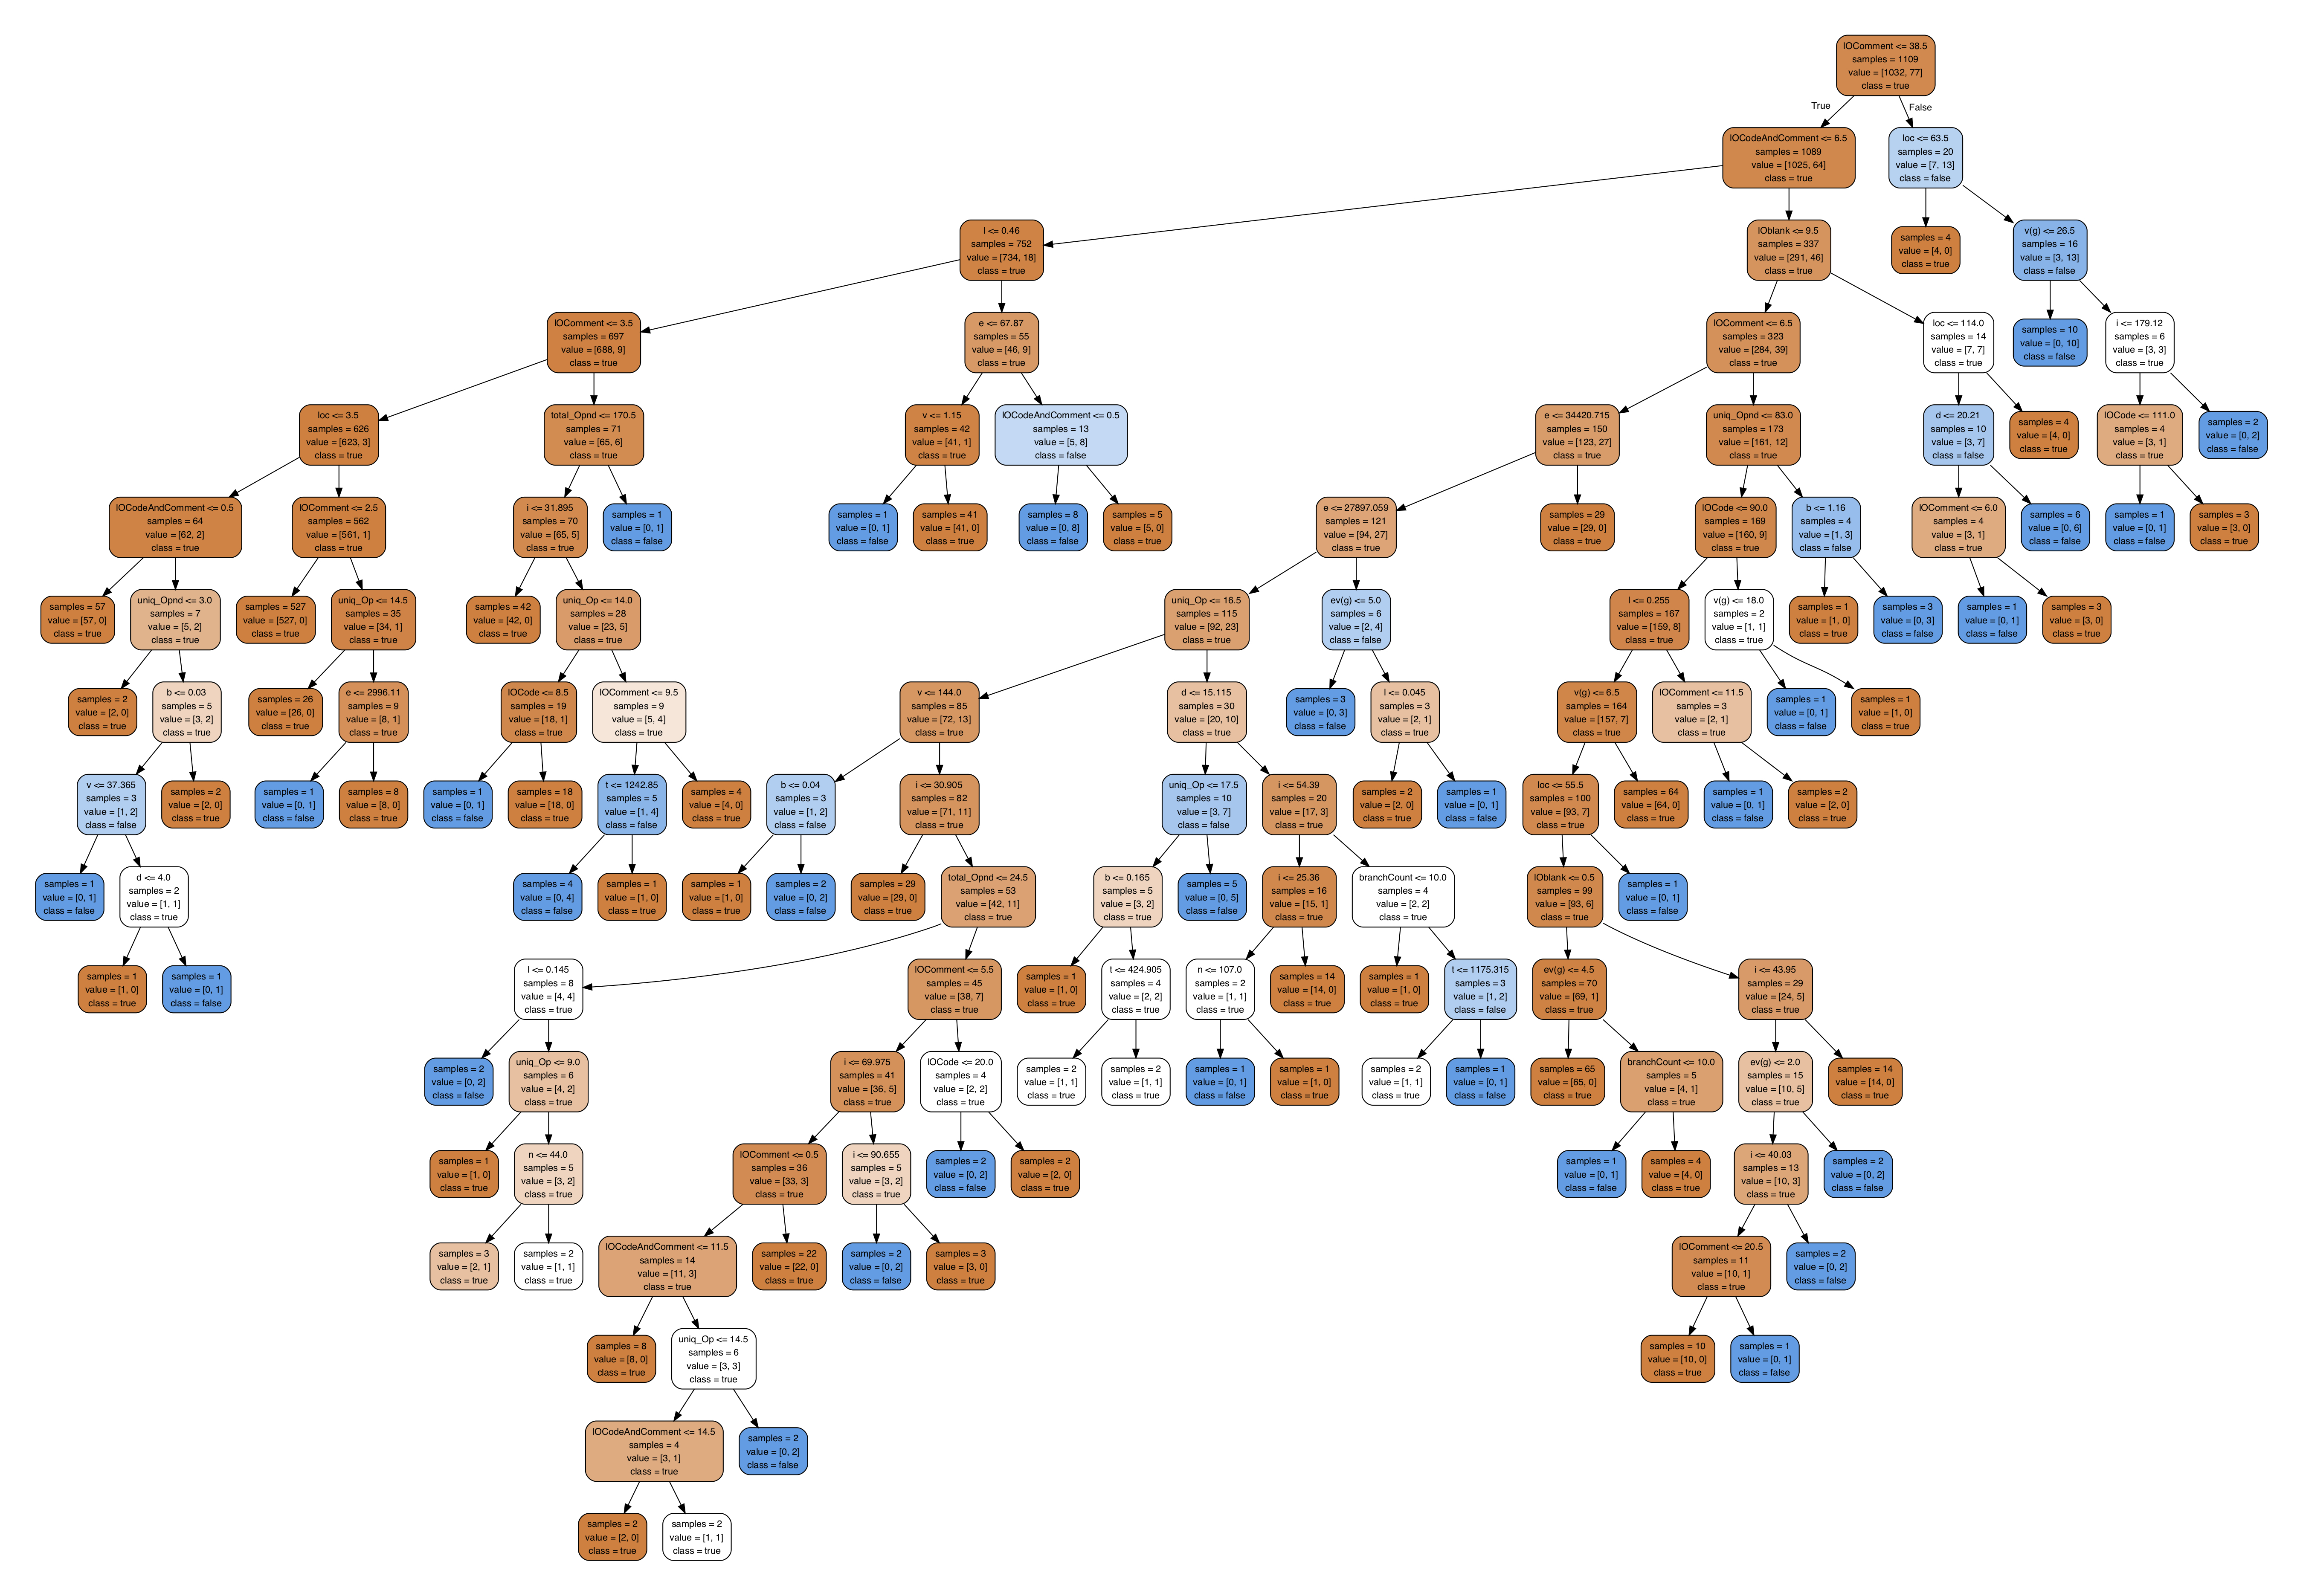
\includegraphics[scale=0.118, angle=90]{img/tree}
    \caption{Sprendimų medžio tipo besimokanti mašina sudaryta naudojant PC1 duomenų rinkinio poaibį}
    \label{img:tree}
\end{figure}


\section{Eksperimentinio palyginimo rezultatai}
% tablesgenerator.com - converts calculators (e.g. excel) tables to LaTeX
\begin{table}[H]\footnotesize
  \centering
  \caption{Lentelės pavyzdys}
  {\begin{tabular}{|l|c|c|} \hline
    Algoritmas & $\bar{x}$ & $\sigma^{2}$ \\
    \hline
    Algoritmas A  & 1.6335    & 0.5584       \\
    Algoritmas B  & 1.7395    & 0.5647       \\
    \hline
  \end{tabular}}
  \label{tab:table example}
\end{table}

\end{document}
